\documentclass[12pt]{article}
\usepackage{graphicx}
%\documentclass[journal,12pt,twocolumn]{IEEEtran}
\usepackage[none]{hyphenat}
\usepackage{graphicx}
\usepackage{listings}
\usepackage[english]{babel}
\usepackage{graphicx}
\usepackage{caption} 
\usepackage{hyperref}
\usepackage{booktabs}
\usepackage{array}
\usepackage{amsmath}   % for having text in math mode
\usepackage{listings}
\lstset{
  frame=single,
  breaklines=true
}
  
%Following 2 lines were added to remove the blank page at the beginning
\usepackage{atbegshi}% http://ctan.org/pkg/atbegshi
\AtBeginDocument{\AtBeginShipoutNext{\AtBeginShipoutDiscard}}
%


%New macro definitions
\newcommand{\mydet}[1]{\ensuremath{\begin{vmatrix}#1\end{vmatrix}}}
\providecommand{\brak}[1]{\ensuremath{\left(#1\right)}}
\providecommand{\norm}[1]{\left\lVert#1\right\rVert}
\newcommand{\solution}{\noindent \textbf{Solution: }}
\newcommand{\myvec}[1]{\ensuremath{\begin{pmatrix}#1\end{pmatrix}}}
\let\vec\mathbf

\begin{document}

\begin{center}
\title{\textbf{Coordinate Geometry}}
\date{\vspace{-5ex}} %Not to print date automatically
\maketitle
\end{center}

\setcounter{page}{1}



\section*{10$^{th}$ Maths - Chapter 7}

This is Problem-7 from Exercise 7.1

\begin{enumerate}

\item The point on the $x$-axis which is equidistant from $\myvec{2 \\ -5}$ and $\myvec{-2\\9}$\\

\solution The input parameters for this problem are available in 


  If $\vec{x}$ lies on the  $x$-axis and is  equidistant from the points $\vec{A}$ and $\vec{B}$, 
\begin{align}
 \norm{\vec{x}-\vec{A}} &=
\norm{\vec{A}-\vec{B}} 
\\
 \implies \norm{\vec{x}-\vec{A}}^2 &=
\norm{\vec{x}-\vec{B}}^2 
\end{align}
which can be expressed as 
\begin{multline}
%  \label{eq:norm2d_dist}
 \brak{\vec{x}-\vec{A}}^{\top} \brak{\vec{x}-\vec{A}}=
 \brak{\vec{x}-\vec{B}}^{\top} 
\brak{\vec{x}-\vec{B}}
\\
 \implies \norm{\vec{x}}^2-2{\vec{x}}^{\top}\vec{A} + \norm{\vec{A}}^2
 \\= \norm{\vec{x}}^2-2{\vec{x}}^{\top}\vec{B} + \norm{\vec{B}}^2
\end{multline}
which can be simplified to obtain
%  \eqref{eq:norm2d_equidist}.
  \begin{align}
   \vec{x} &=
    x\vec{e}_1
  \end{align}
  where 
  \begin{align}
   x &=\frac{\norm{\vec{A}}^2 -\norm{\vec{B}}^2 }{2\brak{\vec{A}-\vec{B}}^{\top }\vec{e}_1
}  
  \end{align}
  now substituting the A and B values in eq.5
\begin{align}
 \brak{\vec{A}-\vec{B}}^{\top}=
 \brak{\myvec{2 \\ -5}-\myvec{-2\\9}}^{\top}
 =\myvec{4 & -14}
\end{align}
  \begin{align}
   \norm{\vec{A}}^2 = 21
    \end{align}
 \begin{align}
   \norm{\vec{B}}^2 = 85
    \end{align}
upon   substituting the values in eq 5. the value of x= $ -7$
\\Hence, the desired point is $\myvec{ -7 \\ 0}$.

\begin{figure}[!h]
 \begin{center}
  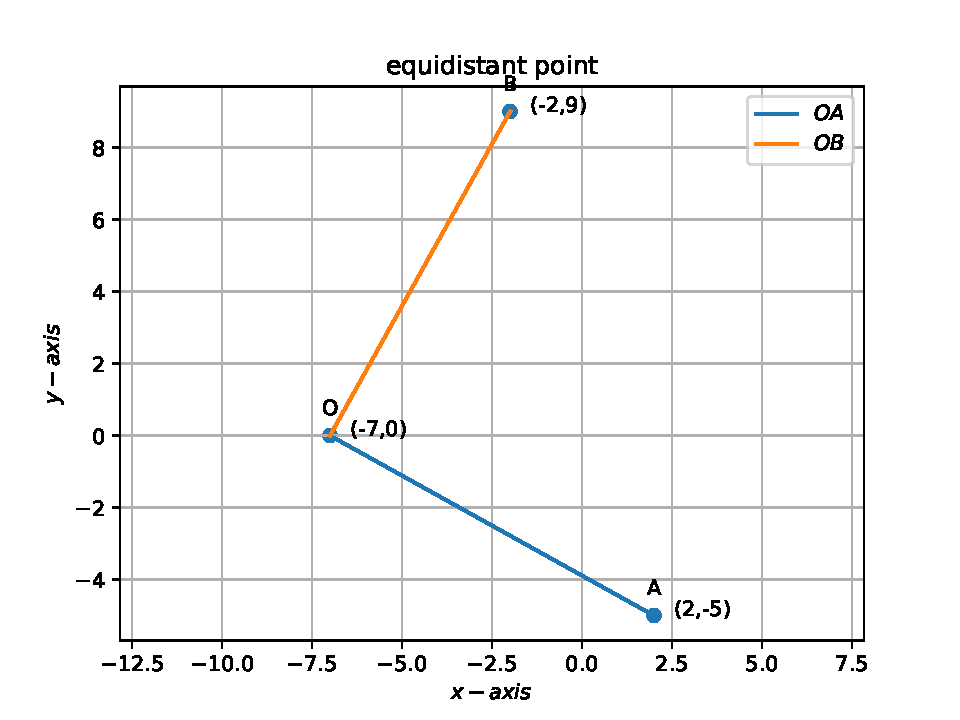
\includegraphics[width=\columnwidth]{./figs/fig.pdf}
 \end{center}
\caption{}
\label{fig:Fig1}
\end{figure}

\end{enumerate}

\end{document}
